% Example template for using the unmeethesis style
% This example is for a Master's candidate in Mathematics
% It contains examples of front matter and most sections that the
% typical graduate student would need to include
% By: N. Doren 02/10/00
%     Minor mods by N. Doren 08/26/11

% Use the following specification for BOTTOM page numbering:
\documentclass[botnum, fleqn]{unmeethesis}
\usepackage{amsmath}
\usepackage{amsfonts}
\usepackage{amsxtra}
\usepackage{amssymb}
\usepackage{mathrsfs}
\usepackage{bm}
\usepackage{xspace}
\usepackage{graphicx}
\usepackage{epstopdf}
\usepackage{multirow}
\usepackage{array}
\usepackage{url}
\usepackage{color,soul}
\usepackage{float}
\usepackage{listings}
% Use the following specification for TOP page numbering:
% \documentclass[fleqn]{unmeethesis}
\def \marhes{{\sc Marhes~}}

\begin{document}

\frontmatter
\title{Automatic Targeting, Point-to-Point Laser Communication System for small robots.}
\author{Paul Groves}
\degreesubject{M.S., Electrical Engineering}
\degree{Master of Science \\ Electrical Engineering}
\documenttype{Project}
\previousdegrees{B.S., Computer Engineer, University of New Mexico, 2012}
\date{May, 2105}
\maketitle
\makecopyright
\maketitleabstract %(required even though there's no abstract title anymore)

\begin{abstract}
There is a need for secure point-to-point communication between robots. The purpose of this project is to create a system to allow secure, point-to-point, laser communication between the pairs of robots. The use of lasers to communicate the message will guarantee that only an agent on the laser's path will be able to intercept the communication under most operating conditions. The system will be designed to be modular in order to be customized to the robot capabilities. A prototype that includes an automatic identification and targeting system is developed and demonstrated. 

\end{abstract}

%\tableofcontents
%\listoffigures
%\listoftables
\mainmatter
\section*{Introduction} \label{chp:introduction}
Wireless communications system are notoriously easy to eavesdrop on. For instance, for home networks the most advanced encryption techniques can be defeated with easily attainable tools \cite{wireless_vulnerabilities}.  When more robust encryption and security techniques are used, such as military applications, just the act of transmitting over radio waves can give valuable information to an attacker, such as the location of the transmitter\cite{wireless_triangulation}.

Laser communications are inherently point-to-point, the message being transmitted can only be read when an agent is in the laser's path, significantly reducing possible attack vectors. Laser systems have been used for point-to-point communications, for example in \cite{nasa_laser}\cite{transportable_laser}. However, these systems use large, specialized, lasers and actuators. The goal of this project is to develop a system that will allow two agents to communicate over a laser beam in the lab, using off the shelve components fitted to the robot's size and load capacity.

The  \marhes Lab specializes in small, autonomous, ground and air based mobile robots. The current systems include Turtlebots from Clearpath Robotics, Octoroaches developed at UC Berkeley, a “Panzer” unit developed in the \marhes Lab, and Quadrotors from AscTek Inc. The laser communication system and prototype are focused on these robots. Smaller robots, such as the Octoroach, will have only a laser receiver module; while larger robots, like the Turtlebot, will have a laser module capable of sending and receiving a message. This gives an operational envelope, in terms of power requirements and weight, that will cover all four platforms present in the \marhes lab.

\clearpage

\section*{System Overview}

A laser communication module will consist of the following components:

\begin{itemize}
 \item Microcontroller Unit (MCU).
 \item Laser sensor.
 \item Laser and laser driver circuit.
 \item Camera.
 \item Alignment actuators.
\end{itemize}

Only the first two items will be required regardless of robot size. Each robot capable of sending a message will have the laser and camera mounted on an actuated gimbal in order to find and track the target module without affecting the sender robot current trajectory or mission.

In this project, I consider a case where a group of robots have a wireless channel for low security communication and a secure message needs to be transmitted between two robots in the network. The process will follow these general steps:

\begin{itemize}
 \item \textbf{Stage 0:}\\ Sender robot communicates its intention to send a secure message to the target robot.
 \item \textbf{Stage 1:}\\ Sender robot commands laser communication module to find and track the target robot.
 \item \textbf{Stage 2:}\\ If equipped, the target robot commands laser communication module to find and track the sender robot.
 \item \textbf{Stage 3:}\\ The laser communication module on the sender robot performs precise alignment of its laser with the target's laser sensor.
 \item \textbf{Stage 4:}\\ The laser communication module on the sender robot sends the message.
 \item \textbf{Stage 5:}\\ Target robot acknowledges message receipt.
\end{itemize}

\subsection*{Stage 0: Preparation}

Due that the robots will need to align their laser communication modules before the modules can be used effectively, their wireless network channel is used to perform this initial handshaking. After the modules find and identify each other, the operation is handled entirely by the laser communication modules. The initial handshaking could include relative position information to hasten the next stage.

\subsection*{Stage 1: Automatic Targeting and Identification}

Each laser communication module is capable of showing a unique visual pattern which identifies it in the group. For an added measure of security, the pattern can be changed during operation. In the prototype developed, the visual pattern is adjusted using LEDs.

The laser communication module in the sender robot is commanded with finding a target pattern, which does by using computer vision. Once the target is identified, the laser communication actuators will continuously track the target robot until the secure communication is completed. 

\subsection*{Stage 2: Reciprocal Alignment}

If the target robot has an actuated laser communication module, it will use it to point its sensor in the direction of the sender robot. If the target robot does not have an actuated laser communication module, their trajectories might be affected in order to perform the alignment. 

\subsection*{Stage 3: Precise Laser-Sensor Alignment}

Once the tracking and base laser-sensor alignment are completed, a precise alignment phase is completed which includes turning the laser on and receiving a visual feedback from the target robot. In the prototype developed, the visual feedback is given by a LED that turns on when the precise alignment has been accomplished measured by the intensity of the laser on the sensor. Depending on the terrain conditions and smoothness of the robot trajectories, the robots might need to stop for the duration of the message to ensure a consistent alignment.

\subsection*{Stage 4: Message Sending}

The message is sent using the laser-sensor pair. Once properly aligned and started, the input of the laser and the output of the sensor will behave like a physical cable while the signal is within the capabilities of the driver and sensor. As the baud rate increases, the error on the message interpretation is increased.

\subsection*{Stage 5: Acknowledgment}

After the message is received, the target robot acknowledges by using the wireless network and the robots continue with their mission.

\section*{Prototype Hardware}\label{chp:}

\section*{Agent}
The agent current is a TurtleBot. The interface to the laser communication module is through the USB port on the TurtleBot computer. Power is provided in the base of the TurtleBot at 12 Volts DC, separate regulators are used to provide power to the various modules. 

\begin{figure}[ht]
 \begin{center}
  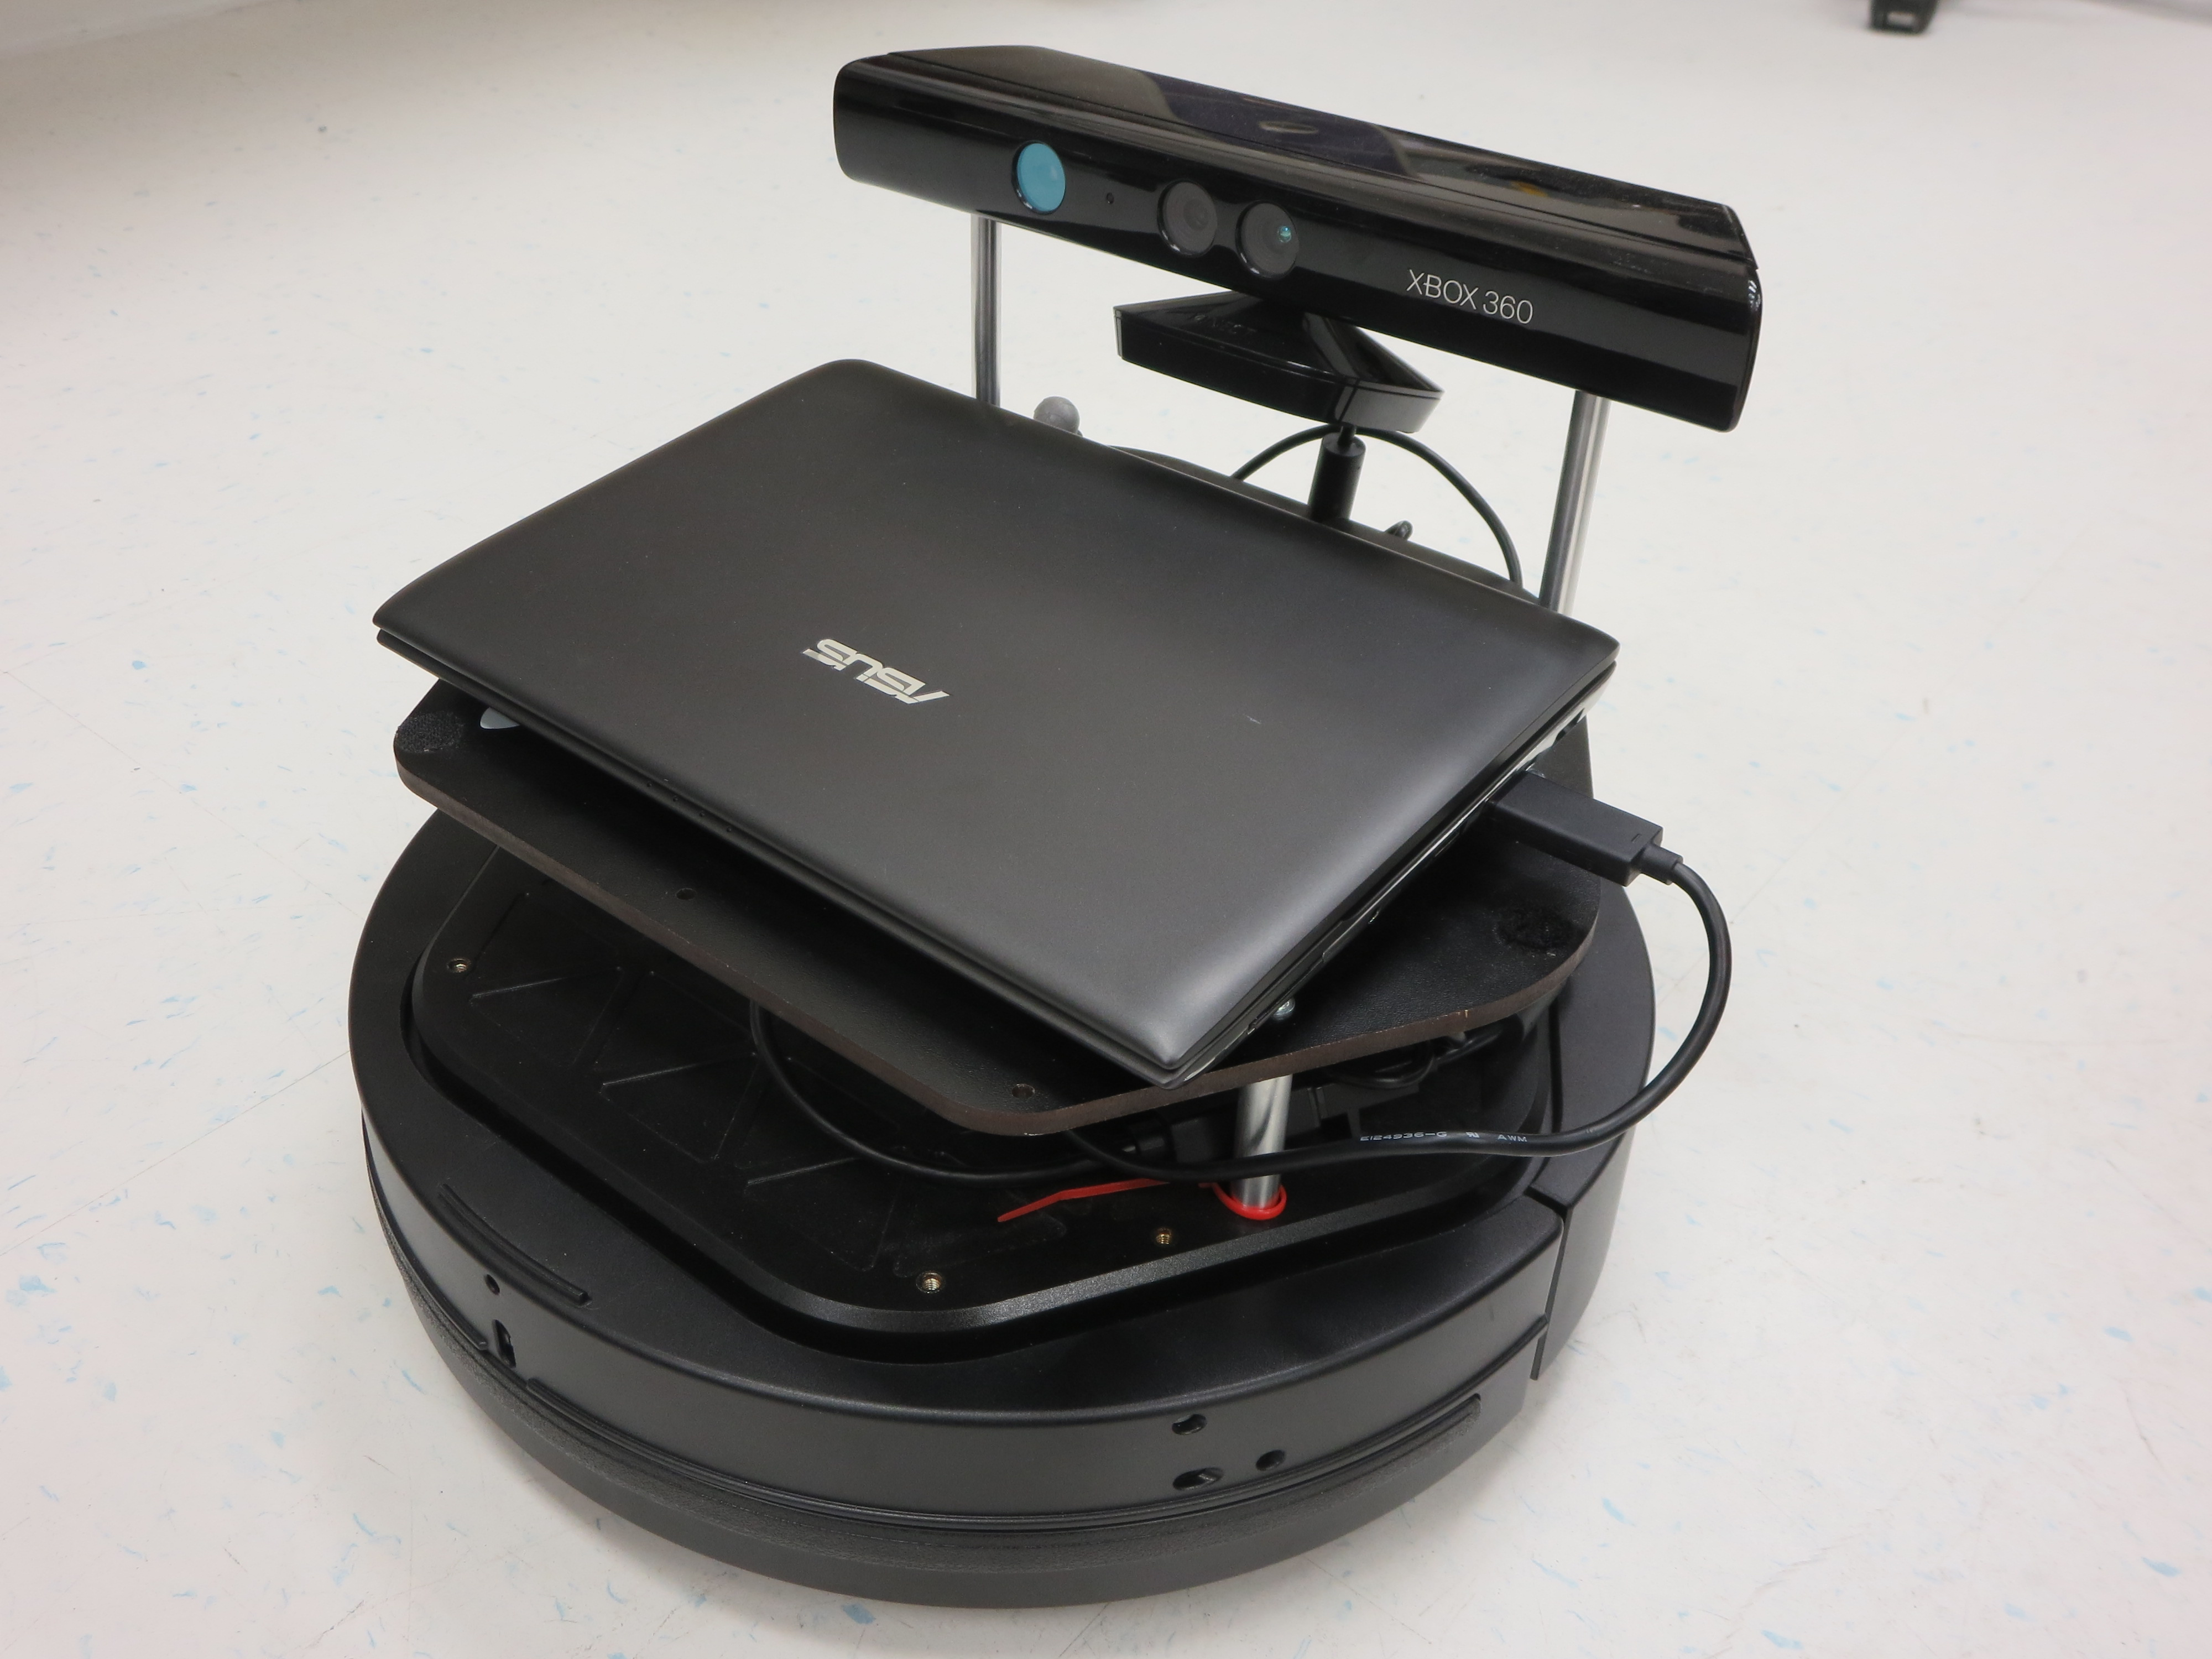
\includegraphics[width=0.5 \textwidth]{figures/TurtleBot.JPG}
  \caption{\small \label{fig:turtlebot} TurtleBot Robot}
 \end{center}
\end{figure}


%\prototype
\subsection*{Microcontroller Unit (MCU)}
The MCU being used is the Intel Edison. The Edison platform has a dual core 500 MHz atom processor, 1 GB of on board memory, and 4 GB of storage. In addition it includes WiFi, Bluetooth, a USB port for power and to provide a console port, and a USB OTG port. 

\subsection*{Alignment Actuator System}
The platform designed incorporates a gimbal system designed and built in house. It uses DC motors connected to an on-board motor PWM (Pulse Width Modulation) driver and H-Bridge.

The gimbal System is composed of two aluminum frames. A coordinate frame fixed to the laser is defined with the Y axis in the same direction as the laser beam and the Z axis pointing up. From the starting position, the internal frame can perform a full 360 degree rotation around the Z axis when actuated by the top motor. The electronics housed in the internal unit consist of the camera, the laser, the laser sensor, the signal strength visual feedback LED, and a cluster of 4 LEDs used for identification. The external frame allows for a +/- 15 Degree rotation about the X axis when actuated by the side motor.

The motors are Polulu Micro Metal with a gear ration of 150:1. They are driven by a Polulu Junior dual DC motor driver. The driver is controlled through a serial port using the standard Polulu command set. It is capable of delivering 2.5A of continuous current at voltages from 5V up to 24V. They are operated at 12V for improved torque.

\subsection*{Laser and Sensor}
The current laser operates in the 450 nM wavelength and is a standard laser pointer type. It is powered from 5 volts DC through transistor driver circuit. Since it can be set to always active, it provides a means of visible confirmation during testing. 

The laser sensor is based on a photodiode. It was selected to match the wavelength of the laser. When the laser strikes the photodiode current flows through it and into the input of the OpAmp. If sufficient current is allowed to pass through to drive the voltage at the pin above the negative input then OpAmp output will be pulled high. The threshold voltage is selectable by adjusting a variable potentiometer. 

The output from the OpAmp goes directly to the MCU. The voltage level is selectable by the pullup voltage at the output pin.

\subsection*{Camera}
The camera being used for development is a GoPro Hero3+. It is a Wifi camera capable of full HDMI resolution with a 90 FOV. 

\section*{System Configuration}

\subsection*{Embedded Platform}
The Edison operates on a Debian 3.2 Headless kernel built from the Yocto project. It includes special libraries from Intel to support access to the extra features of the platform, such as GPIO ports and ADC ports. 

\subsection*{Development Environment}
Main developing was done in Python and C. Python 2.7 was used in this project. The Python libraries were used:

\subsubsection{Computer Vision: OpenCV}
OpenCV is a mature, robust, computer vision library available to the Open Source community. It implements some of the most advanced computer vision algorithms available. OpenCV 2.x was installed onto the Debian image directly from the apt repositories with the following command:
\subsubsection{Camera Driver: GoProHero}
The Hero3+ camera is controlled by connecting to its Ad Hoc network on the camera itself. To interface to the camera an open source tool, GoProHero, was used. It is available on \cite{goprohero}.
\subsubsection{Math: NumPy}
Allows scientific computing and matrix operations.

\section*{Results}

The algorithm under design needs to accomplish several tasks. It must identify a target in the image returned by the camera. It must be able to align the target to the center of the image. And it must then be able to align the laser with the receiver on the target. The algorithm developed allows the hosting agent to command the Laser Communications Module to align the laser onto the targets receiver and send a message over the link.

\subsection*{Target Acquisition Algorithm}

When operating, images are captured every 250 ms. They are transmitted by the GoPro as a Base64 encoded string. This string is decoded into binary values and put into a NumPy array. This array is converted to HSV values and image correction is applied to correct for image aberrations from the GoPro camera. OpenCV's built in Sift algorithm is used to search for the target agent. Once identified a region of interest is created around the detected agent. The distance between the center of the image and the detected agent is used as an error term for the gimbal control. Once this error approaches zero the image is monitored for the signal strength visual feedback LED. A small error around the central region, in the form of a Levy Walk, is used to search for the precise alignment of the laser. Once the signal strength visual feedback LED is detected, motor movement ceases. The desired message is transmitted over the UART to the Laser Encoder / Decoder board. 

\begin{figure}[ht]
 \begin{center}
  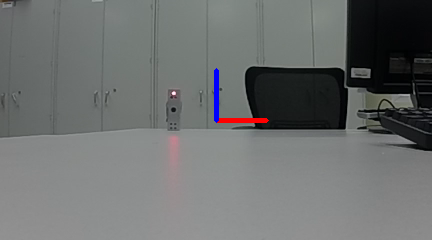
\includegraphics[width=0.5 \textwidth]{figures/frame.png}
  \caption{\small \label{fig:frame} Raw camera image}
 \end{center}
\end{figure}

\begin{figure}[ht]
 \begin{center}
  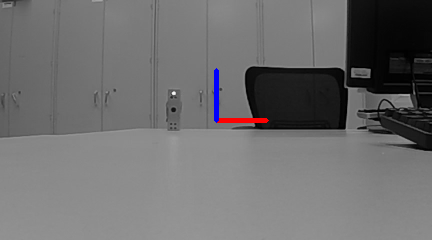
\includegraphics[width=0.5 \textwidth]{figures/bw.png}
  \caption{\small \label{fig:bw} Red channel only from raw camera image}
 \end{center}
\end{figure}

\subsection*{Visual Closed-Loop Control}

The error term for the control equations is derived from the camera images. Once the target is identified the distance to the center of the image is calculated and this result is converted to millimeters. Once the image is centered the Signal Good LED is monitored to determine correct alignment. A small error input is used to cause oscillation about the center of the screen until the Signal Good LED is illuminated. At this point motor movement will cease and the signal is sent. Figure \ref{fig:dot} shows the position of the current center with respect to the target position (white circle).

\begin{figure}[ht]
 \begin{center}
  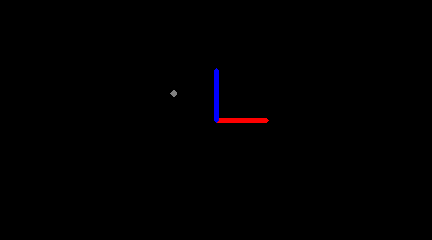
\includegraphics[width=0.5 \textwidth]{figures/dot.png}
  \caption{\small \label{fig:dot} Location of desired target with respect to current center}
 \end{center}
\end{figure}


\subsection*{Target Identification with Thresholding}
Thresholding is the simplest way to track an object. It works in scenarios where the relative brightness of an object is unique in the scene. The LEDs used for identification where purposely selected to allow for just this case. OpenCV is used to perform a thresholding operation, masking out all other areas of the image whose brightness is less than the thresholded value. Once this is done then the openCV command <blah> is used to find connected regions. Since only the LEDs should be left in the image it should also be the only regions identified. The number of regions identified is the target ID. Since 4 LEDs are used for identification, but 2 are needed to be active for centering of the image, a total of 3 targets can be identified using this method.

\subsection*{Target Centering}
The centroid of the identified region is found by using moments algorithm. Based on the ID of the target, the center of these regions is calculated and subtracted from the center of the image. An additional offset is applied, to allow for calibration of the laser and detector positions. This offset is fed into the motor control laws and the process is repeated until the image is centered.

\subsection*{Laser Alignment}
Centering of the target will move the laser close to the photodetector but will probably not strike close enough to activate it. Therefor a Laser Alignment stage is necessary. At this stage the Signal Good LED will be searched for. It should be above the ID LEDs and will also be detectable with thresholding. If the LED is not illuminated then a small random offset will be applied to the center of the image. Once the Gimbal has moved the image to the new target center the LED is checked again. This process is repeated until the LED turns on.  At this point the message is sent across the laser to the target.
%<Images of Signal Good and Mask>


\section*{Future Work} \label{sec:Future Work}


\bibliographystyle{IEEEtran}
\bibliography{ref_paul}

\end{document}
